\documentclass[12pt]{article}

%%%%% Preamble

%% Packages to use

\usepackage{amsmath,amsfonts,amssymb}   %% AMS mathematics macros
\usepackage{graphicx} %% Package to import images.
\usepackage{pagecolor}% http://ctan.org/pkg/{pagecolor}
\usepackage{float}


%% Title Information.
\title{dAbacus Resources v0.2.2}
\author{Ibai Basabe}
\date{}           %% By default, LaTeX uses the current date

%%%%% The Document

\begin{document}


\pagecolor{white}

\maketitle

\begin{abstract}

dAbacus solves both the blockchain trilemma and network localization through scheduled parallelization. dAbacus is a peer-to-peer ecosystem of networks that expands the blockchain with added structure solving the double-spending problem while increasing throughput and reducing latency. Here we introduce our initial resource distributions and deployment to help those interested in contributing to the project make informed decisions. With these resources, we focus on building the liquidity infrastructure of the metaverse both at the foundational layer and the application layer. 

\end{abstract}

\tableofcontents
\newpage



\section{Introduction}

\subsection{Note about the Usage of this Document}

This document has been prepared for information purposes only. It is not soliciting any action from the reader. The contents of this document are subject to change.

\subsection{The Beginning }

Since the design and implementation of Bitcoin, digital sources of liquidity are growing at a staggering rate. In \cite{N}, Satoshi Nakamoto introduced the first digital source of scarcity and with it a new source of liquidity that we can now use. Since then, an ever-growing community focuses on strengthening and supporting this young idea and the broader crypto space born from Bitcoin. In the last ten years, people created many peer-to-peer blockchain networks and devoted much time to strengthening and developing. However, much work is left undone. The vision of a distributed financial infrastructure based on digital resources backed by mathematics rules is still in its infancy. For a complete guide to dAbacus' vision and mission, read \cite{B}.

However young this industry is, the early times of Satoshi are gone, and cryptocurrencies have become common and globally known. dAbacus solves vital problems in the industry, such as the blockchain trilemma and network localization. 

As we have seen with other networks, the community gives value to dAbacus' resources. There are several ways to obtain these resources: dAbacus resources can first be obtained during the initial development phase, second through farming and mining, and third through secondary markets. 

We will use dAbacus resources to run the supernet, from transferring to mining, passing by usages that include deploying and governing The Unit and other Edge dApps.


\subsection{Reasons for dAbacus}

This section aims to list all of the reasons why dAbacus exists and why the community is adopting it. dAbacus' resources will drive their value through human interaction. For this value to live, we need to discuss the benefits of an entirely new protocol.

dAbacus exists for a variety of reason summarized in the following three major points:

\begin{enumerate}

\item dAbacus solves the blockchain trilemma: it increases throughput without compromising security or decentralization through a new blockchain parallelization structure called the blocktree.

\item dAbacus solves network localization: dAbacus allows fast confirmations over long distances by enabling subnetworks in the supernet to be mined locally. 

\item dAbacus brings a new model for smart contracts and the broader blockchain applications market with Edge Dapps.

\end{enumerate}

Secondarily there are many global reasons to support a project like dAbacus:

\begin{enumerate}

\item Bitcoin needs a high consensus level to make changes to the protocol. Furthermore, changes can hurt the ecosystem. However, a new project without a previous network can make many improvements without harming the ecosystem.

\item Overall ecosystem throughput and value grows for every new good project which enters the ecosystem. 

\item Using different security models offers protection against failure of weak security in other networks. 

\item dAbacus gives new players in the ecosystem a way of entering as a new network providing opportunities for newcomers and more incredible innovation. 

\item Liquidity provider competition can develop better and better models.

\end{enumerate}

dAbacus also focuses on many minor improvements to the Bitcoin model with an entirely new code base and a wholly new form of deploying dApps based on the new edge computing model. dAbacus brings more throughput of highly secured on-chain transactions and a platform for highly scalable off-chain decentralized cooperation. Given the possible security vulnerabilities of Bitcoin, dAbacus offers new signature schemes and the most advanced hashing standard. With a longer value discovery profile, dAbacus aims to give its users an excellent opportunity to enter or expand their cryptocurrency usage. We will compete for future liquidity and build the talent necessary to become a worldwide liquidity provider.





\section{Resource Economics}

\subsection{dAbacus Resources}

The dAbacus token (ABA) is the primary resource for the supernet. While dAbacus will allow the deployment of dApps in subnets, the main blocktree will contain all ABA transactions. The maximum amount to ever enter circulation is $2^{34}$ ABA.

\subsection{Allocation}

We allocate dAbacus' resources as shown in Figure \ref{fig:allocation}. 

\begin{figure}[h!]
\centering
  \includegraphics[width=5in]{allocation.png}
  \caption{Total allocation.}
  \label{fig:allocation}
\end{figure}

We reserve an amount comparable to the first four years of Bitcoin mining for the initial distribution.  ASICs will likely be used to mine the remaining 50\% of the supply.



\subsection{Vesting}

An amount of the initial dAbacus resources will be vested for the times defined in Figure \ref{fig:allocation_table}. Founders, Early Development, Seed Round, and Development Fund will have vesting schedules. For a base 10 allocation schedule with inflation rate see Figure \ref{fig:allocation_table2}.







\begin{figure}[H]
\centering
  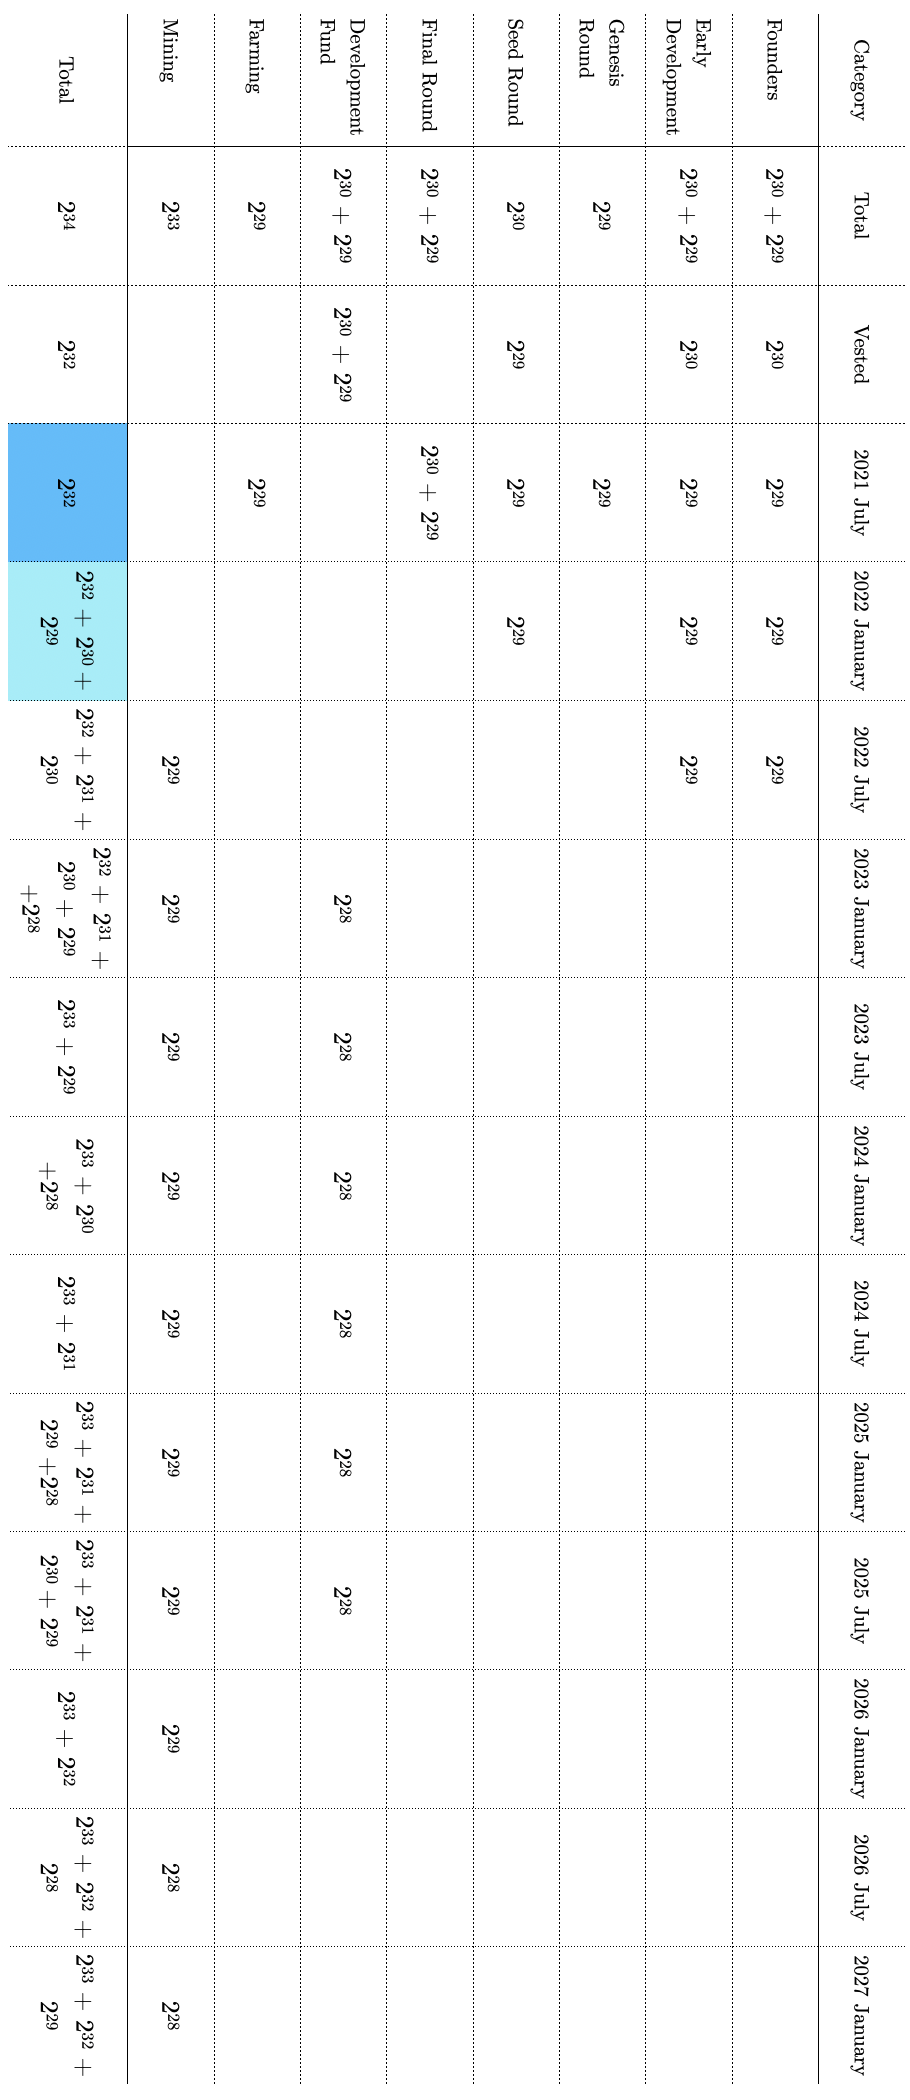
\includegraphics[width=3.5in]{allocation_table.png}
  \caption{Allocation with vesting details}
  \label{fig:allocation_table}
\end{figure}

 \thispagestyle{empty} 

\begin{figure}[H]
\centering
  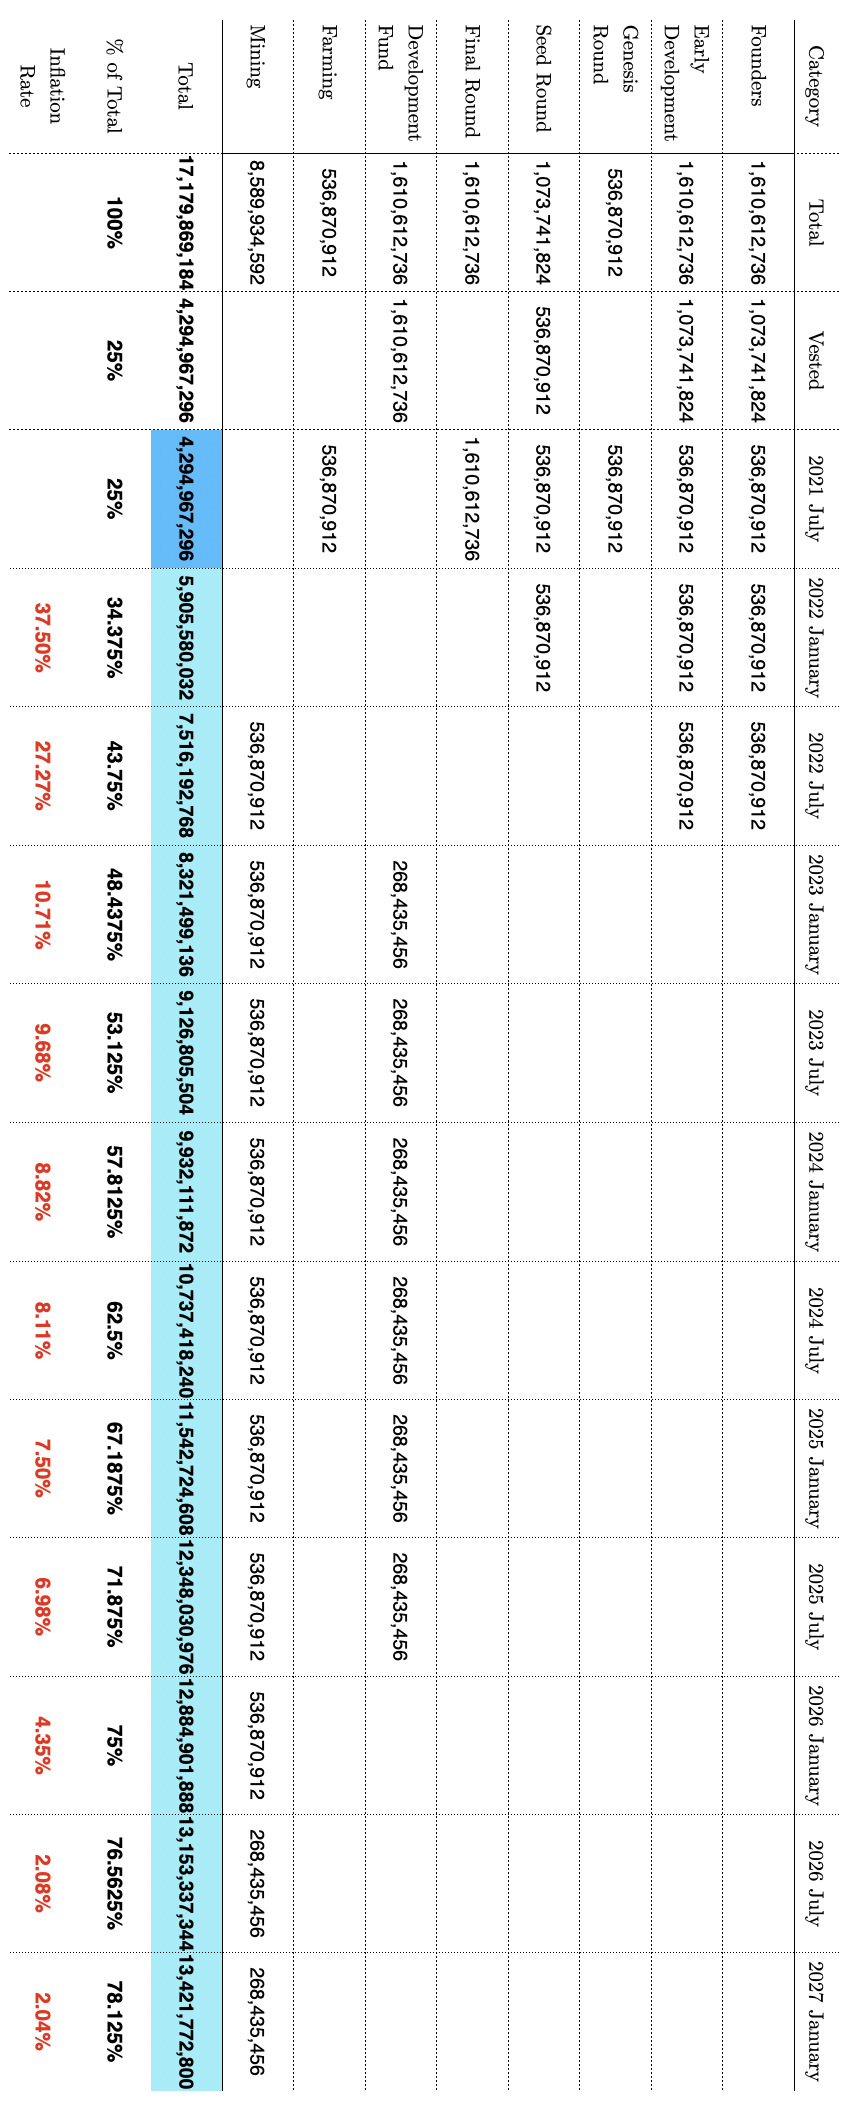
\includegraphics[width=3.5in]{allocation_table_2.png}
  \caption{Allocation details showing inflation rate.}
  \label{fig:allocation_table2}
\end{figure}
 \thispagestyle{empty} 






\section{Development Roadmap}


\subsection{Milestones}

dAbacus' ideas started in February of 2019 after the founder's first 6 years of experience in the crypto industry. Some of the project was started in 2019 but it is in 2021 when the project was carefully organized to execute the plan.

After the launch of The Unit original algorithm on May 5, 2021 (5/5/5), we expect to launch the main net on June 6, 2022 (6/6/6) and launch the capacity to deploy dApps on July 7, 2023 (7/7/7).

The future of dAbacus development is strongly supported by its strategy and the growing community.


\subsection{Community}

dAbacus is a community-driven ecosystem. We are expanding our community in many software development and social platforms to reach a broader and broader set of peers. As we build dAbacus, we encourage the global crypto community to get involved in the governance and the development of both The Blocktree and The Unit as the core implementations of our current roadmap.

The dAbacus community stands by the principles of non-violent communication to create the best possible crypto tools and a vibrant ecosystem of Edge dApps. With The Unit, we are building an essential component of the crypto industry, and the community will ultimately control its governance.

\section{Final Remarks}

The valuing and deployment of dAbacus resources is complex. However, we are building a model and architecture capable of speeding up deployment while increasing efficiency. We have a growing team with sufficient experience to keep driving dAbacus forward. Soon we will all be working for and in the metaverse. 


\begin{thebibliography}{[BLSWZ9]}
\bibliographystyle{amsalpha}

\bibitem[N]{N} Nakamoto, S.: Bitcoin: A Peer-to-Peer Electronic Cash System. \emph{https://bitcoin.org/bitcoin.pdf} (2008).


\bibitem[B]{B} Basabe, I.: dAbacus: Community and Values.
